\section{Introduction}
\label{sec:introduction}


Modern online services are increasingly deployed in multiple geographically-scattered datacenters (geo-replication)~\cite{spanner, kraska2013mdcc, li2012making}. Geo-replication allows services to remain available even in the presence of outages affecting entire data centers   and it reduces access latency by bringing data closer to clients. On the down side, though, the performance of geographically distributed data stores is challenged by the existence of unavoidably large communication delays between datacenters: two datacenters on opposite sides of the earth incur a minimal latency of 133ms, which is utterly bounded by the speed of light and can not be further reduced~\cite{bailis2013highly}. 

The inherently large synchronization overheads that affect geo-replicated data stores has a deep impact on the performance of the protocol employed to enforce data consistency. The problem is particularly exacerbated in partially-replicated data-stores that aim at ensuring strong consistency semantics, i.e., ACID transactions --- two features that are recognized as highly desirable to enhance, on the one hand, system's scalability~\cite{xxx}, and simplify, on the other hand, applications' development. 

For this class of systems, in fact, some form of global synchronization, typically based on a Two-Phase commit protocol scheme~\cite{xxx}, is unavoidable in order to safely detect conflicts developed among  concurrent transactions executing at different data-centers. The adverse impact on performance of inter-data center synchronization is of a twofold nature: i) system's throughput can be severely impaired, as  transactions need to hold locks during their global validation phase, which can cripple the effective concurrency that these systems can achieve; ii) client-perceived latency is also directly affected, since the inter-data-center  synchronization phase lies in the critical path of execution of transactions.


%This has motivated the investigation of a broad spectrum of data replication protocols for geo-replicated systems~\cite{xxx} as well as the exploration of diverse trade-off regarding the  consistency semantics offered to application developers~\cite{xxx}.

This work focuses on investigating the opportunities and challenges associated with the use of \textit{speculative} processing techniques in geo-distributed partially replicated transactional data stores  that provide a widely employed consistency criterion, i.e., Snapshot Isolation~\cite{xxx}. Generally speaking, speculative transactional processing techniques aim at avoiding to block transaction processing in presence of potential conflicts with other concurrent transactions (possibly executing at remote data-centers) by making an optimistic assumption on how  such conflicts will be eventually resolved.

More in detail, we distinguish between two classes of speculative transaction processing techniques, which we call \textit{internal} and \textit{external} speculation depending on whether their effects are transparent or not for the programmers.

{\bf REVIEWED UP TO HERE}


. Internal speculation techniques are completely transparent to the programmers, in


With the term ``internal speculation'' we refer to a set of (distributed) concurrency control techniques that speculate on the outcome of concurrent transactions in order to avoi



or replicated transaction

 of integrating speculative tec

 focuses on the  of a set of speculative transaction processing techniques, 

In this class of systems, where inter-replica synchronization has a dominant cost





Data stores that embrace strongly consistent semantics, like Scatter~\cite{scatter} and Google's Spanner~\cite{spanner} are reckoned~\cite{shute2012f1} to greatly reduce the complexity of building distributed applications by providing programmers with the powerful abstraction of ACID transactions. However, it is also well known~\cite{brewer2012cap}  that enforcing strong-consistency requires introducing the latency of several inter-datacenter network round trips along the critical path of transactions' execution. This has not only a direct impact on the user-perceived latency --- a key discrimination factor for online services and a potential cause of large revenue losses  \cite{schurman2009user}, but also on throughput. In fact, throughout the execution of the replica synchronization protocol --- typically based on a Two-phase commit scheme~\cite{spanner,peluso2012score} --- existing strongly consistent data stores maintain, so called, pre-commit locks on the data items accessed by transactions. The duration of these locks, in geo-distributed data stores, can easily last on the order of a few hundreds of milliseconds. As a consequence, in workloads that generate non-minimal data contention, the probability of incurring lock convoying effects is greatly amplified, which can severely hinder the maximum throughput the system can withstand.

In order to tackle this problem, several systems have resorted to use weak consistency models, such as eventual consistency~\cite{kawell1988replicated, lloyd2011don, cure}, which allow to propagate transactions (or even individual operations, in case transactions are not supported) asynchronously. This brings remarkable benefits in terms of user-perceived latency and achievable throughput. These benefits, though, come at the cost of a significant increase of complexity for the application developers, who have to take responsibility of enforcing application's correctness in spite of a broad range of subtle concurrency anomalies~\cite{shute2012f1}. This includes developing compensation logic for transactions whose output has been externalized, in a speculative fashion, without waiting for the completion of the global certification phase: e.g., in an e-commerce application, handling the scenario in which a purchase order has to be eventually rejected or emended because the last stock of some requested item has been attributed to a concurrent transaction. Moreover, weak consistency models also require programmers to ensure that the application's logic does not break when transactions observe non-atomic snapshots that reflect only partially the effects of concurrent transactions or non-isolated snapshots that reflect the effects of conflicting transactions. This type of anomalies can be quite hard to predict or reason about, as they manifest as subtle concurrency bugs that can lead to anomalous system states, e.g., divisions by zero or infinite cycles~\cite{guerraoui2007opacity}, that may compromise the safety of user level applications, e.g., crashing them, and from which it is typically impossible to recover using business-level compensation logic.
\iffalse
In order to tackle this problem, in the literature various trade-offs have been explored between programming complexity and system performance by weakening the consistency semantics provided to programmers. some systems totally remove cross-site synchronous operations~\cite{kawell1988replicated, lloyd2011don, cure}; some reveals preliminary results to users to reduce latency, before operations finish execution~\cite{planet, icg}, and some systems that mix multiple consistency levels to reduce the latency of commutative operations~\cite{redblue, PSI}. Weakening system consistency brings remarkable benefits in terms of user-perceived latency and achievable throughput. These benefits, though, come at the cost of a significant increase of complexity for the application developers, including dealing with subtle concurrent anomalies, analyzing applications and writing compensation logics to emend the side-effect of externalized speculative results. 
\fi

%caused by observing data snapshots not producible by any sequential execution of transactions
\begin{figure}
\centering
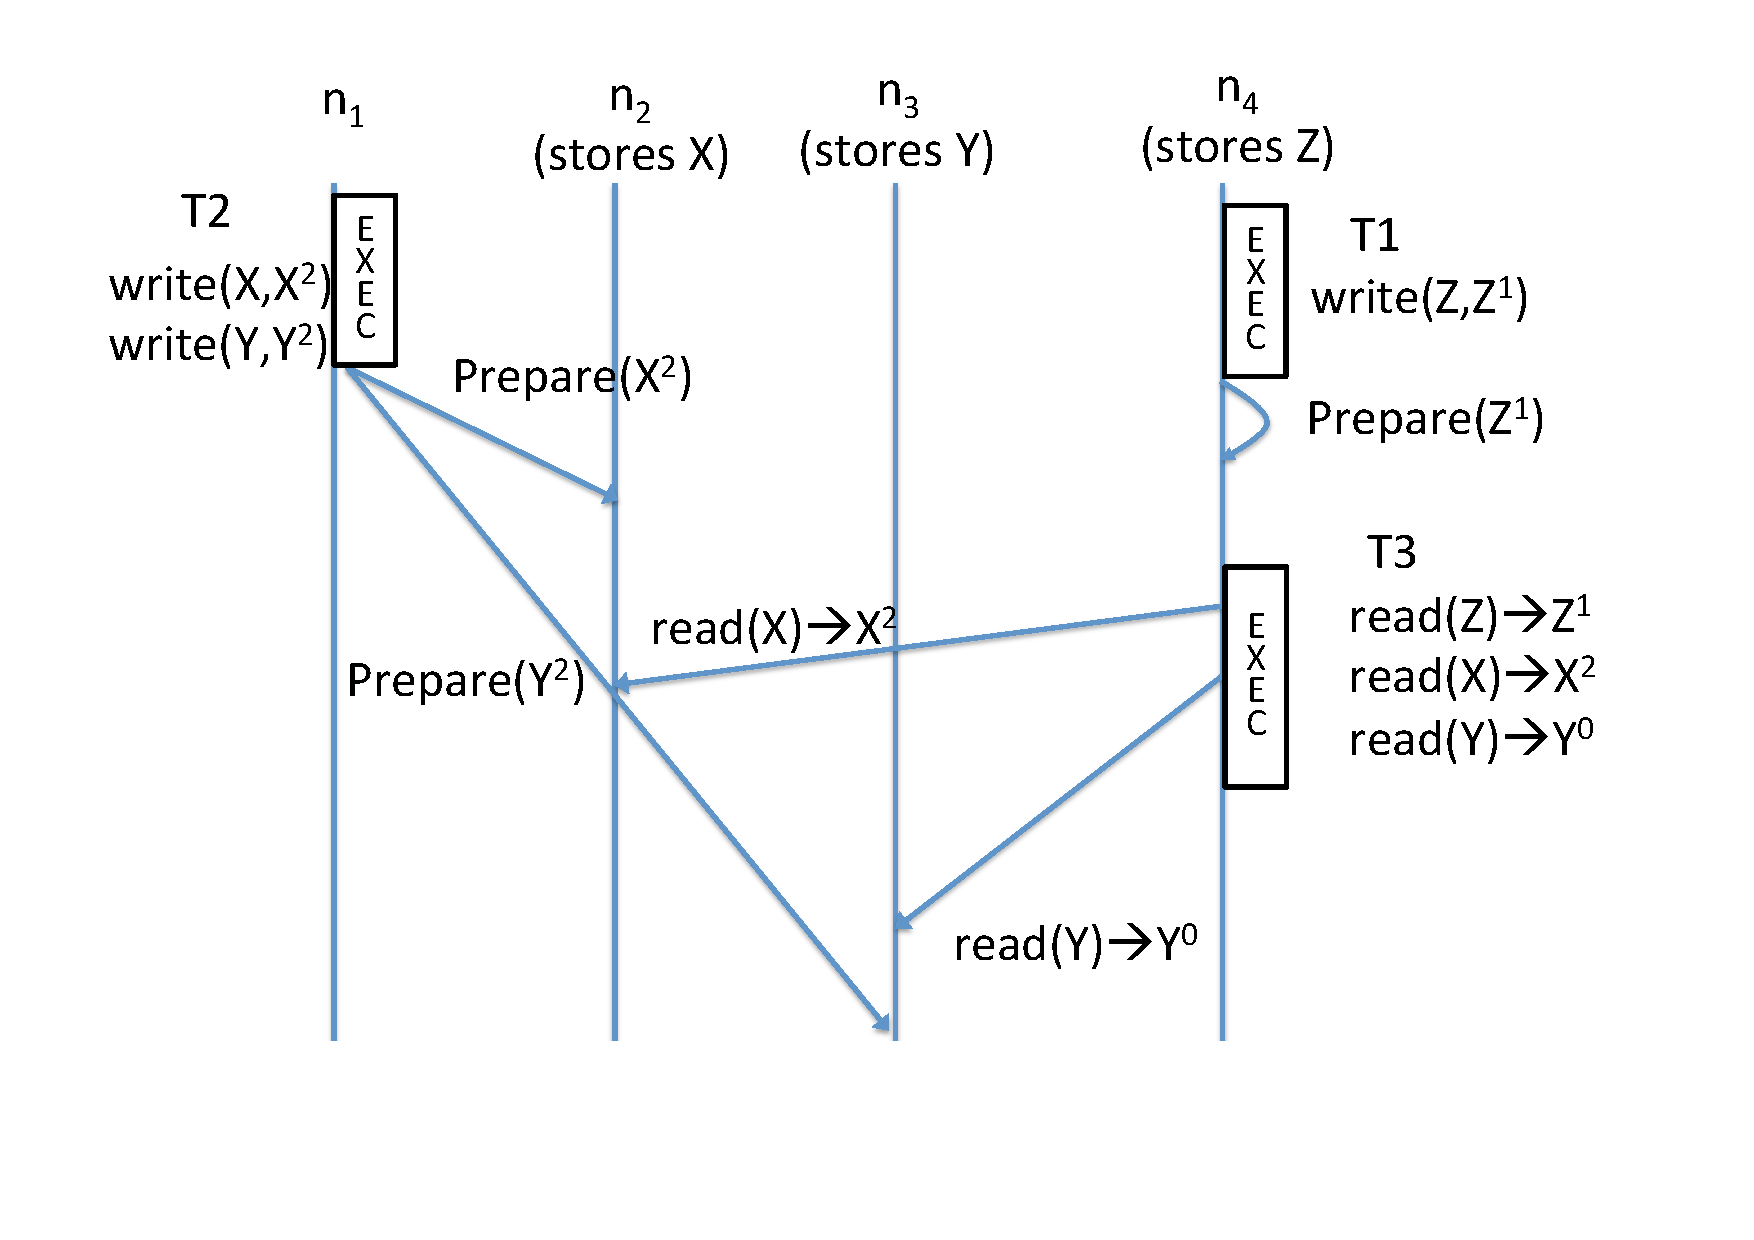
\includegraphics[scale = 0.24]{figures/example.pdf}
\caption{\footnotesize Example concurrency anomaly that may arise when adopting weak-consistency models that do not abide by the SPSI criterion.}
\label{fig:example}
\end{figure}

The system proposed in this paper, which we called \specula (Speculative Transactional Replication), provides developers with the flexibility of choosing between two different consistency semantics for the transactions that compose their applications: a strong consistency semantics, i.e., the familiar Snapshot Isolation~\cite{berenson1995critique}, and a weakly consistent one, which we termed Speculative Snapshot Isolation (SPSI). The idea of unifying different consistency models within the same programming model is not new: two notable examples are the red-blue consistency model recently proposed in Gemini~\cite{li2012making} and the support in SQL for specifying different isolation levels on a per transaction basis~\cite{sqk}.  The main innovative aspect of \specula lies in its novel transactional replication protocol, which provides unique advantages with respect to state of the art systems that provide either strong or weak consistency semantics (or both).

~\\
\noindent {\bf Strong consistency semantics:} 
\iffalse
The protocol employed by \specula to ensure strong consistency shares several key design choices with state-of-the-art data stores~\cite{spanner,clock-si,PelusoScore}, which contribute to its efficiency and scalability. These include:  multi-versioning, which maximizes efficiency in read-dominated workloads~\cite{bernstein-book},  distributed clocks, which are used to establish the transaction serialization order in a fully decentralized fashion,~\cite{spanner} as well as support for partial replication, a  feature that is generally regarded as fundamental to achieve high scalability~\cite{kemmeAndRicardo,PelusoGMU}. 
\fi
\specula supports transactions with strong consistency semantics, i.e. Snapshot Isolation, which provides programmers the familiar ACID properties. However, comparing with conventional transactional protocols, \specula takes a radically different approach regarding the management of transactional conflicts involving pre-committed data. Existing strong-consistent protocols take a conservative approach, which prevents any transaction T from ever observing the data item versions pre-committed by a different transaction T' --- either by blocking T till T' commits, or by letting T observe the pre-image of the execution of T'. This choice is arguably motivated by the fact that allowing transactions to observe pre-committed data item versions exposes them to the risk of cascading aborts~\cite{xxx}, a property that is ``historically'' deemed as crucial to maximize the efficiency of a transactional system~\cite{textbooks-on-db}. \specula departs from these conventional designs, and embraces a speculative approach that spares transactions that incur a conflict on pre-committed data from having to wait for the finalization of the commit phase of the lock-holding transaction. Conversely, \specula's distributed concurrency control mechanism takes an optimistic approach, i.e., it speculates on the eventual success (i.e., commit) of pre-committed transactions and allows the data versions pre-committed by a transaction T to be read by concurrent transactions, that are hence speculatively serialized after T. As we will show via an extensive experimental study, \specula's design choice of allowing speculative read can lead to increase throughput by up to XX$\times$ and reduce latency by up to YY$\times$. A striking, and more general, result stemming from our work is that, in strongly consistent geo-replicated data stores, the advantages stemming from accepting the risk of cascading aborts largely outweighs its drawbacks, leading to remarkable gains in terms of both throughput and latency.

~\\
\noindent {\bf Weak consistency semantics:} Analogously to the well-known eventual consistency model~\cite{brewer2012cap}, the weak consistency model supported by \specula, i.e., SPSI, allows application developers to \textit{speculative commit} transactions, i.e., to externalize to its users (e.g., human operators) the results of a transaction while this is still undergoing its final commit/certification phase. As such, when programmers choose to exploit the speculative commit capabilities of \specula, they also need to develop compensation logic for coping with the case in which a speculatively committed transaction has to be eventually aborted.

What distinguishes SPSI from existing weak consistency models is that it provides clear and stringent guarantees on the atomicity and isolation of the snapshots observed and produced during transactions' execution. Figure~\ref{fig:example} illustrates one of possible concurrency anomalies that can arise in a transactional system that adopts weak consistency, by exposing the data item versions produced by speculatively committed transactions: transaction T3 observes the version of data item X precommitted by a concurrent transaction, T2, on node n$_1$. However, when it comes to reading Y, which was also updated by T2, T3 misses the version created by T2 on node n$_3$ (as T2's updates are still being propagated to node \textit{n$_2$}). Such concurrency anomalies are prevented by the SPSI specification, which, in a nutshell, guarantees that the snapshots that can be observed/speculatively committed by a transaction T originated at a node \textit{n}
%
% observable by \textit{any} transaction (independently of whether they ) and those that are produced by a speculatively committed transaction T 
% 
 are equivalent to the ones that would have been observed/committed by T, had it been executed by a non-speculative SI data store along with a subset of all the transactions existing in the system, which excludes any concurrent, speculatively committed transaction originated at a node $n'\neq n$.
% 
% 
%  
% 
%  processed a subset of the entire set of transactions existing in the system that does include specu which comprises all the transactions that, by the time T started,  i) had either finalized their commit phase or ii) were activated on the same node that originated T and had speculatively committed.
 On the one hand,  SPSI  spares programmers from complex concurrency bugs, by ensuring that  transactions always execute on snapshots that are atomic and isolated, although not capturing the effects of concurrent, speculatively committed remote transactions. On the other hand, by demanding that the snapshots over which transactions execute reflect \textit{only} the effects of locally activated concurrent transactions, SPSI's specification allows for efficient implementations that can decide whether it is safe to speculatively commit a transaction solely on the basis of local information.

%, as illustrated in the example execution in Figure~\ref{example}, and ii) it makes transactions subject to cascading-aborts~\cite{xxx}, a property that is ``historically'' deemed as important for the efficiency of a transactional system. \specula rules out the former risk, thanks to an innovative, fully distributed, multi-versioned concurrency control scheme
%
%such data item to be ever observed, by blocking the  transaction requesting access to the data item or
%
%, though, departs from one of the key a
%
%
%
%Still, the latency and performance cost for guaranteeing consistency results seems indispensable. For example, logically a banking system should always be execute with strong consistency, as monetary loss caused by inconsistent operations seems unacceptable \cite{li2012making}. Interestingly, this is not always the case for systems used in daily life. Brew et al. described the design of a practical automated teller machine (ATM): when an ATM experiences network partition, it indeed takes the risk of overdrafting accounts to allows withdrawal unilaterally. In fact, ATM's ability to dispense money outweighs the trouble caused by account overdraft. Accidental overdraft will be handled by a well-defined external compensation logic \cite{brewer2012cap}.
%
%The design of the described ATM comes from a profound insight: practical applications may not always need 100\% consistency guarantee; instead, as long as the latency and availability benefit pay off the cost of compensating occasional mistakes, they may take risks, i.e. speculate on the result of operations, instead of pessimistically waiting out uncertainty \cite{helland2009building, brewer2012cap, bailis2013eventual}. In light of this, this paper presents {\specula}, a distributed transactional key-value store that exploits speculation to circumvent the inherent large latency and low throughput of strongly-consistent transactions. The main goal of \specula is to endow application developers the flexibility to speculate transactions for latency and throughput, while keeping programming complexity in check.
%
%\specula consists of a programming interface and a speculative transaction protocols. The programming interface allows programmers to exert control over speculative transaction: programmers develop application with strong consistency by default, but also have the choice to specify transactions to execute in a speculative fashion, without affecting other transactions. \specula 's speculative transactional protocol enables efficient transaction processing and ensures meaningful semantics, namely SPeculative Snapshot Isolation (SPSI), to programmers. Previous research works have exploited different aspects of speculation execution \cite{kraska2009consistency, pang2014planet}: Consistency Rationing \cite{kraska2009consistency} proposes cost models to measure the best tradeoff of consistency and cost; PLANET \cite{kraska2009consistency} proposes a speculative programming interface and calculates the commit probability of transactions. However, to the best of knowledge, we are the first to propose a speculative transactional protocol for modern large-scale, fully decentralized datastore.
% &  111 &  Haha &  Stupdi &  Noway & ahaha &   \\ \hline

Overall, this paper makes three main contributions:
~\\
\noindent {\em 1.} We propose SPeculative Snapshot Isolation (SPSI), a consistency criterion ad hoc designed for speculative transactional systems. SPSI extends the notion of Snapshot Isolation in an intuitive way, in order to provide meaningful consistency guarantees to transactions observing speculatively committed data (\S \ref{sec:overview}, \ref{sec:protocol}).
~\\
\noindent {\em 2.} We present the design of \specula, a  geo-replicated data store that exploits a novel, fully-decentralized, highly scalable protocol that efficiently supports speculatively transaction execution in presence of partially-replicated data  (\S \ref{sec:protocol}).
~\\
\noindent {\em 3.} We conduct an extensive experimental evaluation (\S \ref{sec:evaluation}),  encompassing both complex/realistic benchmarks (TPC-C and Rubis) and synthetic micro-benchmarks that allow us to exercise a wide range of diverse workloads. The results of our study highlight that:
\begin{itemize}
\item \specula's innovative speculative concurrency control ensures strong consistency (SI) with  average  gains of XX\% in throughput and YY\% in latency with respect to state of the art systems, with peak gains that extend up XX$\times$ for throughput and YY$\times$ for latency. 
\item Applications that adopt \specula's weak consistency semantics (SPSI) can reduce the user-perceived latency, on average  (i.e., considering both scenarios of successful and unsuccessful speculation), by an additional XX\% factor. Further, \specula's weak consistency semantics   allow for enhancing the throughput achievable by \specula by up to XX$\times$ in machine-to-machine applications in which the rate of submission of new transactions is solely throttled by the speed at which the system can process previously submitted transactions.
\end{itemize}

The remainder of this paper is structured as follows. {\bf TODO}

